\documentclass[UTF8]{ctexart}
\usepackage[]{ctex}
\usepackage{natbib}
\usepackage{graphicx}
\usepackage{enumitem}
\usepackage{setspace}
\usepackage{float}
\bibliographystyle{plain}

\title{过定点最短路并行编程报告}
\author{杨景凯 520021910550}
\date{2022年 5月 13日}

\begin{document}

\begin{center}
    \quad \\
    \quad \\
    \kaishu \fontsize{45}{17} 上\quad 海\quad 交\quad 通\quad 大\quad 学
    \vskip 3.5cm
    \heiti \zihao{2} 过定点最短路并行编程\\
    实验报告
\end{center}
\vskip 3.5cm
\begin{quotation}
    \songti \fontsize{30}{30}
    \doublespacing
    \par\setlength\parindent{12em}
    \quad 
\begin{center}
    学\hspace{0.61cm} 院:\underline{电子信息与电气工程学院}

    学生姓名:\underline{\qquad    \quad \quad 杨景凯    \quad  \quad\qquad }

    学\hspace{0.61cm} 号:\underline{\quad \quad\quad520021910550\quad\quad}
\end{center}
    \centering
    2022年5月13日
\end{quotation}

\clearpage
\tableofcontents

\clearpage
\section{背景介绍}
\subsection{实验背景}
最短路问题是图论理论的一个经典问题,就是在指定图网络中找一条从起点到终点间权重
最小的一条路径,解决这类问题的经典算法有 Dijkstra、Floyd 等。

最短路问题在实际生活中有非常广泛的应用。考虑这样一个具体的实际场景:幸运的上海
交通大学学生源源在某天同时抢到了麦当劳、超市、小眷村等的购买机会,于是他需要从宿舍
出发去购买对应的食物,如果只考虑路上的距离,哪条路径可以从宿舍出发,经过以上所有地
点后再回到宿舍,且需要走的路最短呢?\cite{refpdf1}

本次实验是在使用 Dijkstra 算法完成上述最短路任务后,结合多线程优化时间,并比较分析多线程的优化效率。

\subsection{实验环境}
本次实验环境如下:
\begin{table}[H]
    \centering
    \begin{tabular}{|c|c|}
        \hline
        项目 & 参数\\
        \hline
        CPU型号 & AMD Ryzen 5 4600H\\
        \hline
        CPU核心数 & 6\\
        \hline
        CPU线程数 & 12\\
        \hline
        CPU L1缓存容量 & 8192KB\\
        \hline
        系统 & WSL2-Ubuntu20.04\\
        \hline
    \end{tabular}
    \caption{实验环境}
\end{table}

注:该CPU采用了超线程技术(HT),使得线程数多于核心数。

\section{方案设计}
\subsection{并行理由}
本次实验我主要针对Dijkstra算法进行多线程优化。原因如下:
\begin{itemize}
    \item 我首先对所有在part1中的数据进行时间统计,分别统计了使用Dijkstra算法计算最短路的时间以及遍历所有全排列找最短距离的时间。发现在大多数情况下,均为Dijkstra算法需要时间更久。
    \item Dijkstra算法更适合并行,因为它适合拆分成许多块,且各个块之间数据互不干扰。
    \item 对于每一个中间节点,计算最短路的时间是大致相同的,只要给每个线程分配的中间节点数目相近,那么就会使得每个线程时间大致相同。
\end{itemize}

因此本次实验我主要针对Dijkstra算法进行多线程优化。

\subsection{并行思路}
假设中间节点有N个,多线程数目为M,我有以下两种并行思路:
\begin{itemize}
    \item 每个线程使用的中间节点在中间节点集合中位置为非连续的。
    \item 每个线程使用的中间节点在中间节点集合中位置为连续的。
\end{itemize}

在第一种情况下,每个线程所搜索的数目是不固定的,每个线程搜索的起点为$i$,$i$为线程序号。
在这种情况下,存在两个问题:
\begin{itemize}
    \item 各线程长度不一定相同,由于木桶效应,最终速度取决于最长的时间,造成结果不准确。
    \item 由于不连续,使得增加了不必要的CPU缓存MISS,使得性能下降。
\end{itemize}

而第二种情况下,每个线程所搜索的数目是固定的,为$N_{blocknum}=\lfloor N/M \rfloor$。在另外一个子线程中运行剩余的部分,而剩余的部分长度小于其他子线程中长度,因此不会对结果造成影响同时保证了实验的准确性。同时,连续的片段也减少了CPU缓存的MISS几率。

综上,本次实验中,我采用了第二种并行思路。

\subsection{代码细节}
假设中间节点有N个,多线程数目为M。代码详细步骤如下:

1. 使用std::vector<std::thread>来记录所有线程。

2. 计算得到每个线程搜索的数目。$N_{blocknum}=\lfloor N/M \rfloor$。

3. 使用thread创建M个线程,并将线程存于std::vector<std::thread>中(引用的变量使用std::ref()函数得到)。

4. 线程函数接受6个参数,分别如下:

\begin{itemize}
    \item int begin:表示开始的位置。开始位置为$i \cdot N_{blocknum}$,$i$为线程序号。
    \item int end:表示结束的位置。结束位置为$i \cdot N_{blocknum}+N_{blocknum}-1$,$i$为线程序号。
    \item vector<int> \&intermediates:引用的参考工具vector,不需要占用额外内存,表示中间节点集合。
    \item vector<vector<int$>>$\&length:引用的vector,不需要占用额外内存,表示需要计算出的所有的最短路径长度。
    \item vector<vector<vector<int$>>>$\& allpath:引用的vector,不需要占用额外内存,表示需要计算出的所有的最短路径。
    \item FixedSP* fixedsp:表示调用该函数的对象指针,方便调用其内部的图。
\end{itemize}

5. 每个线程中,从begin至end逐个遍历,调用Dijkstra算法计算最短路。

6. Dijkstra函数接受4个参数,分别如下:

\begin{itemize}
    \item int source:源点。Dijkstra函数将计算从源点出发至其他点处的最短路。
    \item vector<int> \&length:引用的vector,不需要占用额外内存,表示需要计算出的从源点出发的最短路径长度。
    \item vector<vector<int$>>$ \&path:引用的vector,不需要占用额外内存,表示需要计算出的从源点出发的最短路径。
    \item FixedSP* fixedsp:表示调用该函数的对象指针,方便调用其内部的图。
\end{itemize}

\subsection{数据集}
本次实验我采用python生成数据集。测试集中,包含有不同图的大小(节点数目)和不同的中间节点数目。

图的大小采用以下四组:50、100、200、400。

对于每个图,若该图节点数目为$n$,分别采用以下三种测试中间节点数目:$n$、$\lfloor \frac{n}{3} \rfloor$、$\lfloor \frac{n}{5} \rfloor$。同时采用以下特殊中间节点数目:50、100、200、400(如果总节点数大于中间节点数的话)。

对于每种测试图与测试中间节点,分别采用以下线程数目:1、2、4、6、10、12、14、16、20。

每个图均为无向正权路图,且不存在自环。每条路径权值为$0 \sim 1000$的随机整数。

每个中间节点数组均为$0 \sim size(array)-1$的数,且开始节点均为$size(array)-1$。
\subsection{测试方式}
由于为多线程时间测试,不能使用clock()函数,只能朴素地通过本地时间来计算,由于为Linux平台,故使用gettimeofday()函数。

对于每种测试组合,我进行50次测试,计算平均时间。该目的是减少其他进程对时间计算造成的影响。

\section{实验结果}
\subsection{全部数据结果}
全部数据结果表格与详细图像由于过多,故放在了附录位置。以下是全部数据结果的缩略图像。

\begin{figure}[H]
    \centering
    \begin{minipage}[t]{0.45\linewidth}
    \centering
    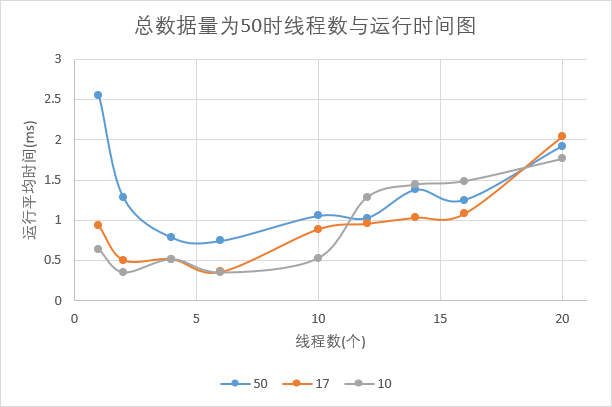
\includegraphics[scale=0.33]{50.png}
    \caption{总数据量为50时运行时间(ms)与线程数(个)图}
    \end{minipage}%
    \begin{minipage}[t]{0.45\linewidth}
    \centering
    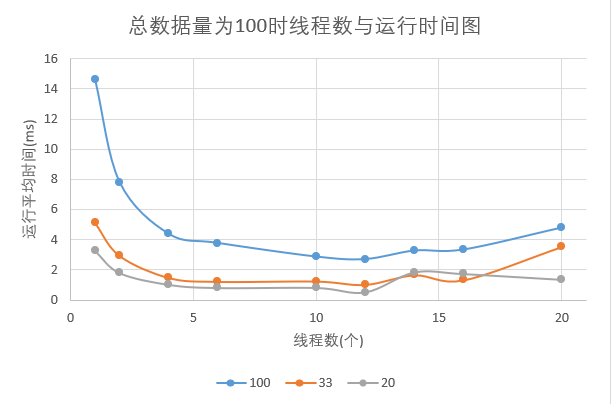
\includegraphics[scale=0.33]{100.png}
    \caption{总数据量为100时运行时间(ms)与线程数(个)图}
    \end{minipage}
\end{figure}
\begin{figure}[H]
    \centering
    \begin{minipage}[t]{0.45\linewidth}
    \centering
    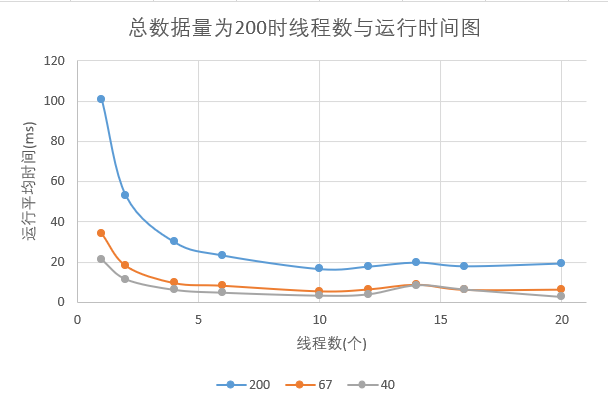
\includegraphics[scale=0.33]{200.png}
    \caption{总数据量为200时运行时间(ms)与线程数(个)图}
    \end{minipage}%
    \begin{minipage}[t]{0.45\linewidth}
    \centering
    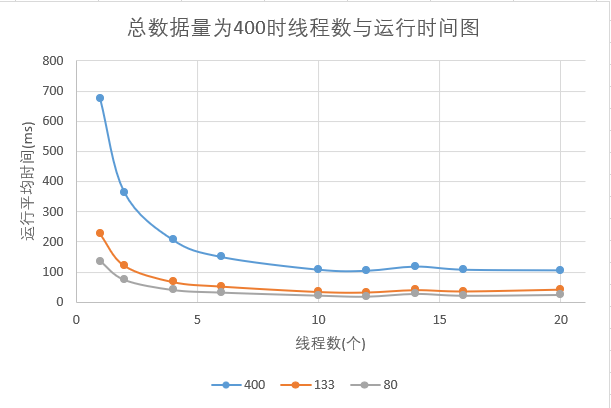
\includegraphics[scale=0.33]{400.png}
    \caption{总数据量为400时运行时间(ms)与线程数(个)图}
    \end{minipage}
\end{figure}


\subsection{运行时间与总数据量关系}
为方便直观地观测效果,我们采用线程数为12,分别对不同中间节点数目统计了运行时间和总数据量的关系。结果如图所示:
\begin{figure}[H]
    \centering
    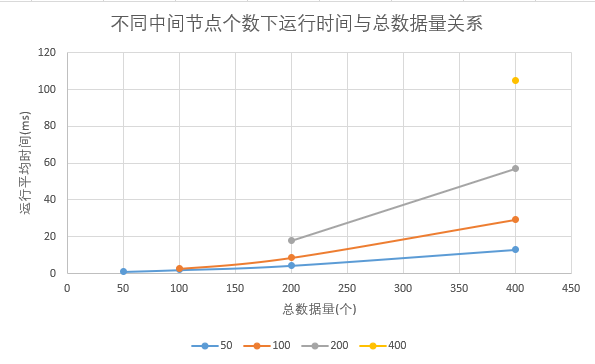
\includegraphics[scale=0.7]{T-totN.png}
    \caption{不同中间节点个数下运行时间(ms)与总数据量(个)关系图}
\end{figure}

通过图像我们可以直观地发现,随着总数据量增加,运行平均时间增加,且近似为多项式型。

\subsection{运行时间与并发程度(线程数目)关系}
为方便直观地观测效果,我们采用总数据量为400和50的数据表格与图像,进行分析。

数据量为400时,数据量偏大,对具有较大数据量的测试具有一定的代表性:

\begin{figure}[H]
    \centering
    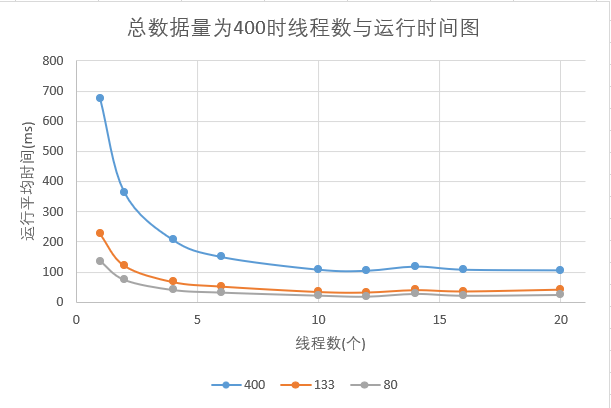
\includegraphics[scale=0.7]{400.png}
    \caption{总数据量为400时运行时间(ms)与线程数(个)图}
\end{figure}

通过图像我们可以清楚地看到,随着线程数的增加,运行平均时间减少。
\begin{itemize}
    \item 在线程数位于$0 \sim 6$ 阶段时,随着线程数目增加,运行时间快速减少。
    \item 在线程数位于$6 \sim 12$阶段时,随着线程数目增加,运行时间缓慢减少。
    \item 在线程数位于$12 \sim 20$阶段时,随着线程数目增加,运行时间处于稳定。
    \item 在线程数为16时,运行时间均出现了小幅度下降。
\end{itemize}

数据量为50时,数据量偏小,对具有较小数据量的测试具有一定的代表性:

\begin{figure}[H]
    \centering
    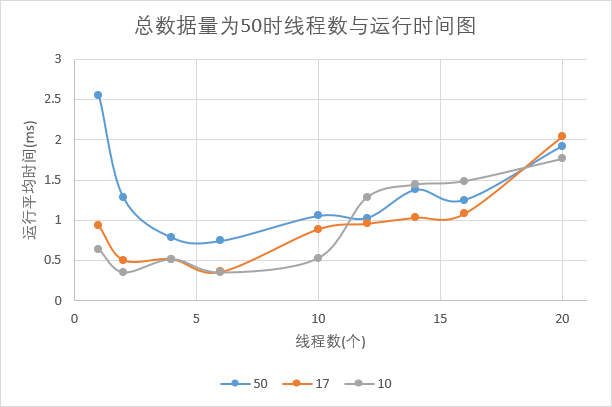
\includegraphics[scale=0.7]{50.png}
    \caption{总数据量为50时运行时间(ms)与线程数(个)图}
\end{figure}

通过图像我们可以清楚地看到,随着线程数的增加,运行平均时间总体先减少,后增加。
\begin{itemize}
    \item 在线程数位于$0 \sim 6$ 阶段时,随着线程数目增加,运行时间总体呈减少趋势。
    \item 在线程数位于$6 \sim 20$阶段时,随着线程数目增加,运行时间波动,甚至上升。
\end{itemize}

\subsection{运行时间与中间节点数目关系}
为方便直观地观测效果,我们采用总数据量为400,分别对不同线程统计了运行时间和中间节点数目的关系。结果如图所示:
\begin{figure}[H]
    \centering
    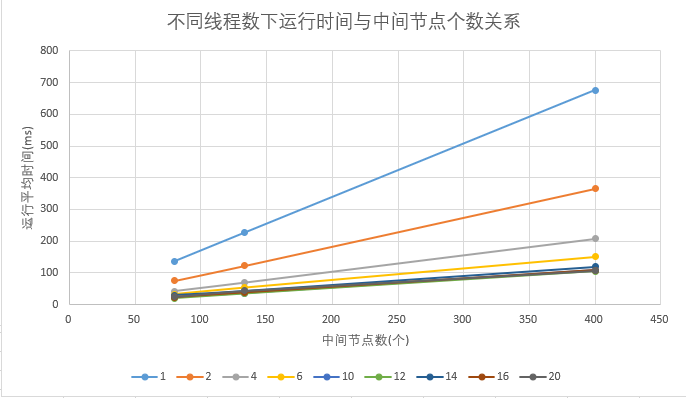
\includegraphics[scale=0.6]{T-N.png}
    \caption{不同中间节点个数下运行时间(ms)与中间节点数(个)关系图}
\end{figure}

通过图像我们可以直观地发现,随着中间节点数增加,运行平均时间增加,且近似为线性。

\section{分析与结论}
\subsection{运行时间与总数据量关系}
对于Dijkstra算法来说,总数据量增加,图中路径增加。两者关系近似满足$N_{path}=N_{node}^2$。因此,当总数据量增加,对于每个源点,搜索路径呈平方式增加。故对于相同线程数、相同中间节点来说,随着总数据量增加,运行平均时间增加,且增加幅度随着总数据量增加而增加。

以上分析与实验结果相同,故实验成功。
\subsection{运行时间与并发程度(线程数目)关系}
对于Dijkstra算法来说,线程数目增加,会带来以下后果:
\begin{itemize}
    \item 当线程数增加时,每个线程内部运行时间缩短,且近似呈反比例关系。
    \item 当线程数位于$1 \sim N_{MAXthreadNum}$(其中$N_{MAXthreadNum}$表示CPU支持最大线程数)时,CPU并行的线程数目等于此时线程数目。
    \item 当线程数多于$ N_{MAXthreadNum}$(其中$N_{MAXthreadNum}$表示CPU支持最大线程数)时,CPU并行的线程数目等于$N_{MAXthreadNum}$。
    \item 每个线程的产生和结束均会产生开销,总开销CPU时间随线程数目呈线性增加。
\end{itemize}

综合以上可以认为,当线程内部运行时间较长时,满足以下两条规律:
\begin{itemize}
    \item 当线程数位于$1 \sim N_{MAXthreadNum}$(其中$N_{MAXthreadNum}$表示CPU支持最大线程数)时,若每个线程运行时间大致相近,那么总运行时间与线程数目近似呈反比例关系。
    \item 当线程数多于$ N_{MAXthreadNum}$(其中$N_{MAXthreadNum}$表示CPU支持最大线程数)时,若每个线程运行时间大致相近,运行时间处于稳定。
\end{itemize}

当线程内部运行时间较短时,满足以下三条规律:
\begin{itemize}
    \item 当线程数位于$1 \sim N_{MAXthreadNum}$(其中$N_{MAXthreadNum}$表示CPU支持最大线程数)时,若每个线程运行时间大致相近,那么总运行时间与线程数目近似呈反比例关系。但是由于线程产生和结束的开销,造成波动或不完全满足反比例关系。
    \item 当线程数多于$ N_{MAXthreadNum}$(其中$N_{MAXthreadNum}$表示CPU支持最大线程数)时,若每个线程运行时间大致相近,运行时间并不会减少,甚至可能由于线程产生和结束的开销而增加。
    \item 由于运行时间较短,造成随机误差偏大,曲线应该处于波动状态。
\end{itemize}

实验中,总数据量为400的每个线程运行时间较长,因此可以对应第一种情况。由于CPU最多线程数为12,我们发现,当线程数处于$1 \sim 12$时,平均运行时间减少,当线程数多于$12$时,平均运行时间处于稳定状态。以上分析与实验结果相同,故实验成功。值得注意的是,当线程数为16时,运行平均时间减少,猜测可能是由于16刚好为2的整数次幂,因此使得操作系统更容易安排上下文交换(context switch)。

实验中,总数据量为50的每个线程运行时间较短,因此可以对应第二种情况。由于CPU最多线程数为12,我们发现,当线程数处于$1 \sim 6$时,平均运行时间减少,当线程数多于$6$时,平均运行时间增加。以上分析在线程数位于$6 \sim 12$时与实验结果不符,我认为原因可能是由于操作系统并不会使得全部线程被短时间就可以进行完的程序占用,而是只调用了全部核心来执行,但是不会启用超线程技术(HT),考虑到核心数为6,因此实验结果合理,实验成功。

\subsection{运行时间与中间节点数目关系}
对于Dijkstra算法来说,中间节点数增加,搜索源点数目增加。两者关系近似满足$N_{source}=N_{internode}$。因此,当中间节点数增加,搜索源点数目呈线性增加,但是对于每个源点来说,搜索路径长度近似保持不变。故对于相同总数据量、相同线程数来说,随着中间节点数增加,运行平均时间呈线性增加,且增加幅度与中间节点数目无关,保持不变。

以上分析与实验结果相同,故实验成功。

\section{总结与致谢}
在进行实验时,我刚开始使用了clock()函数来计时,但是发现随着线程数增加,运行时间均增加。这是不合理的。查询资料得知clock()函数是会统计所有占用CPU的时间,那么自然随着线程数增加,由于线程产生和结束的开销,造成了CPU总占用时间增加。

后来改用了本地时间的方式,使得实验得以成功进行。在此感谢各论坛和博客,尤其是CSDN提供的帮助。

\section{附录}
\subsection{全部数据结果表格}
\begin{table}[H]
    \centering
    \begin{tabular}{|c|c|c|c|c|}
        \hline
        总数据量:50& 	50& 	17& 	10\\
        \hline
        1&	2.55128&	0.92944&	0.63586\\
        \hline
        2&	1.28348&	0.5053&	0.3514\\
        \hline
        4&	0.78454&	0.51782&	0.51522\\
        \hline
        6&	0.7439&	    0.35856&	0.3495\\
        \hline
        10&	1.05462&	0.88836&	0.52924\\
        \hline
        12&	1.02832&	0.95664&	1.28538\\
        \hline
        14&	1.37744&	1.03206&	1.44342\\
        \hline
        16&	1.25166&	1.08028&	1.48722\\
        \hline
        20&	1.91874&	2.03546&	1.76262\\
        \hline
    \end{tabular}
    \caption{总数据量为50时运行时间(ms)与线程数(个)表格}
\end{table}
\begin{table}[H]
    \centering
    \begin{tabular}{|c|c|c|c|c|}
        \hline
        总数据量:100& 	100&	33& 	20\\
        \hline
        1&	14.62634&	5.1304&	3.28492\\
        \hline
        2&	7.81046&	2.94988&	1.81178\\
        \hline
        4&	4.38446&	1.4956&	1.03344\\
        \hline
        6&	3.77682&	1.23872&	0.8215\\
        \hline
        10&	2.87432&	1.25954&	0.82548\\
        \hline
        12&	2.70992&	1.03765&	0.53496\\
        \hline
        14&	3.27218&	1.6687&	1.8573\\
        \hline
        16&	3.3439&	    1.3369&	1.74632\\
        \hline
        20&	4.79652&	3.53796&	1.36686\\
        \hline
    \end{tabular}
    \caption{总数据量为100时运行时间(ms)与线程数(个)表格}
\end{table}
\begin{table}[H]
    \centering
    \begin{tabular}{|c|c|c|c|c|}
        \hline
        总数据量:200& 	200& 	67& 	40\\
        \hline
        1&	100.69814&	34.15362&	21.05566\\
        \hline
        2&	52.86528&	18.0946&	11.4164\\
        \hline
        4&	29.98734&	9.65932&	6.27204\\
        \hline
        6&	23.37806&	8.36064&	4.86346\\
        \hline
        10&	16.62768&	5.58432&    3.41018\\
        \hline
        12&	17.84762&	6.52134&	4.07352\\
        \hline
        14&	19.89596&	8.8878&	8.5548\\
        \hline
        16&	18.04038&	6.31804&	6.44198\\
        \hline
        20&	19.40142&	6.42434&	2.7674\\
        \hline
    \end{tabular}
    \caption{总数据量为200时运行时间(ms)与线程数(个)表格}
\end{table}
\begin{table}[H]
    \centering
    \begin{tabular}{|c|c|c|c|c|}
        \hline
        总数据量:400& 	400& 	133& 	80\\
        \hline
        1&	676.52572&	226.98724&	136.7455\\
        \hline
        2&	364.98054&	122.0321&	74.71334\\
        \hline
        4&	207.29286&	68.36666&	41.54984\\
        \hline
        6&	150.56206&	53.43846&	32.96632\\
        \hline
        10&	108.5518&	35.67364&	22.9499\\
        \hline
        12&	105.00562&	33.96196&	19.5449\\
        \hline
        14&	118.88824&	41.71642&	28.64534\\
        \hline
        16&	108.54252&	37.4595&	22.62028\\
        \hline
        20&	106.32808&	43.38704&	25.19194\\
        \hline
    \end{tabular}
    \caption{总数据量为400时运行时间(ms)与线程数(个)表格}
\end{table}
\clearpage
\subsection{全部数据图像}
\begin{figure}[H]
    \centering
    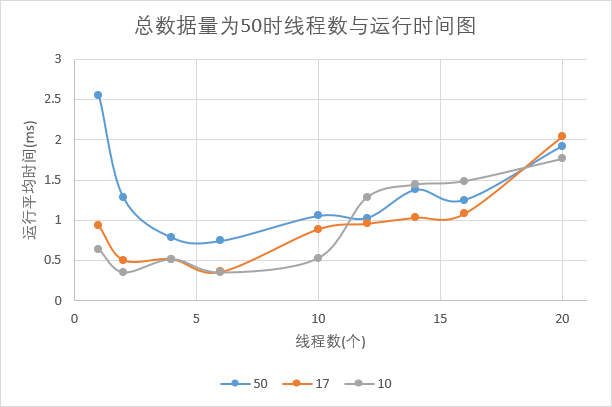
\includegraphics[scale=0.7]{50.png}
    \caption{总数据量为50时运行时间(ms)与线程数(个)图}
\end{figure}
\begin{figure}[H]
    \centering
    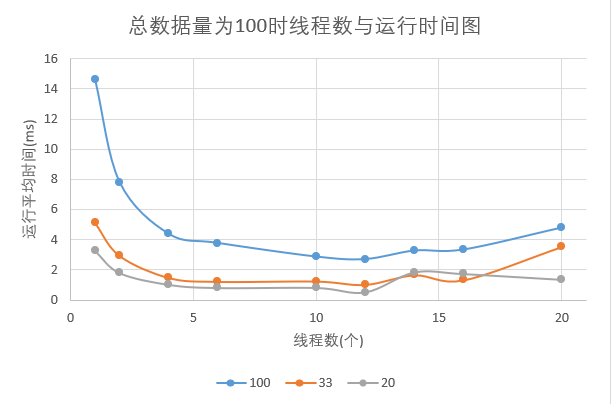
\includegraphics[scale=0.7]{100.png}
    \caption{总数据量为100时运行时间(ms)与线程数(个)图}
\end{figure}
\begin{figure}[H]
    \centering
    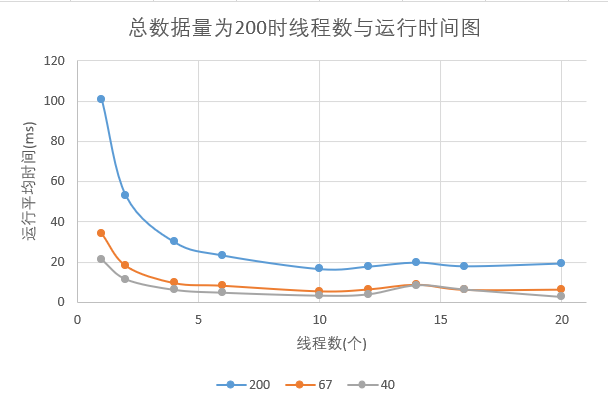
\includegraphics[scale=0.7]{200.png}
    \caption{总数据量为200时运行时间(ms)与线程数(个)图}
\end{figure}
\begin{figure}[H]
    \centering
    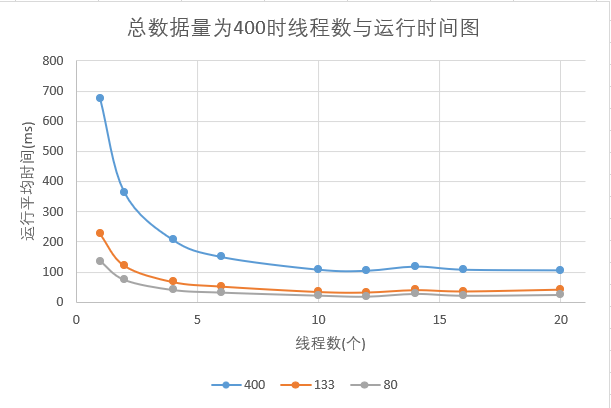
\includegraphics[scale=0.7]{400.png}
    \caption{总数据量为400时运行时间(ms)与线程数(个)图}
\end{figure}
\clearpage
\subsection{运行时间与总数据量关系表格}
\begin{table}[H]
    \centering
    \begin{tabular}{|c|c|c|c|c|}
        \hline
                &50&	100&	200&	400\\
                \hline
        50&	    1.02832	&		& & \\
        \hline
        100&	1.98312&	2.70992	&	& \\
        \hline
        200&	4.32472&	8.62868&	17.84762&	\\
        \hline
        400&	12.91156&	29.2357&	56.96842&	105.00562\\      
        \hline
    \end{tabular}
    \caption{不同中间节点个数下运行时间(ms)与总数据量(个)关系表格}
\end{table}
\clearpage
\begin{thebibliography}{99}
    \bibitem{refpdf1}Lab2.过定点最短路.pdf
\end{thebibliography}

\end{document}
